\begin{apendicesenv}
\partapendices

\chapter{This is a frog}
% Texto do primeiro apêndice.
\label{appendix:frog}
\begin{figure}[H]
    \centering
    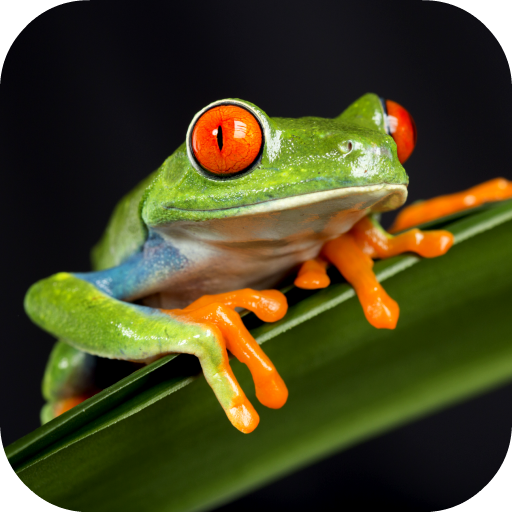
\includegraphics[width=1\textwidth]{figuras/Frog.png}
    \caption{This is a frog}
    \label{fig:frog}
\end{figure}

\chapter{This is another frog}

% Texto do segundo apêndice.
\label{appendix:frog2}
\begin{figure}[H]
    \centering
    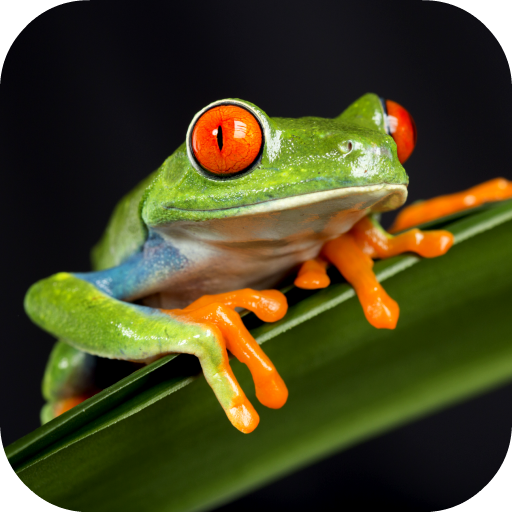
\includegraphics[width=1\textwidth]{figuras/Frog.png}
    \caption{This is another frog}
    \label{fig:frog2}
\end{figure}





\end{apendicesenv}
